% COSC418 Final Presentation
% Regan Gunther and Henry Jenkins - 2011

%\documentclass[handout]{beamer}
\documentclass{beamer}

\usetheme[secheader]{Boadilla}
\usecolortheme{seahorse}
\usepackage[latin1]{inputenc}
\usepackage{mathtools}
\usepackage{listings}
\usepackage{verbatim}
\usepackage{graphics}


\title{COSC418 Project:\\Load balancing in a CTP based network}
\author{Henry Jenkins and Regan Gunther\vspace{20pt} \\
\tiny{(https://github.com/steakunderscore/COSC418-Assignment)}}
\date{September 30, 2011}
\institute[2011]{Department of Computer and Electrical Engineering,\\
    University of Canterbury, \\ Christchurch, \\ New Zealand}

\begin{document}

\frame{\titlepage}

\section[Outline]{}
\frame{\tableofcontents}

\section{Design}
\subsection{Overview}

\begin{frame}
  \frametitle{Our Design}
  \begin{itemize}
    \item $p^* = \text{arg min}  p \in \{\ \text{direct neighbours} \}\
      [\alpha  \cdot (ETX_{s,p} + ETX_p) + \beta \cdot L_p^s]$

    \item Our design is to keep $L_p^s$ locally 
    \item We increment $L_p^s$ as:
    \item $L_p^s = n_p^s - t_p^s$
    \item $n_p^s \geq t_p^s$
    \item Where $t_p^s$ is incremented periodically through a timer
    \item $t_p^s$ is included to stop $L_p^s$ getting too large.
    \end{itemize}
    Why do this instead of transmitting link load data
    \begin{itemize}
    \item Allows us to use the unmodified CTP routing packet
    \item Means we can add load balancing to an existing CTP network
    \item No extra data transmission
  \end{itemize}

\end{frame}

\begin{frame}[fragile]
  \frametitle{UnicastNameFreeRouting}
  
    \begin{itemize}
      \item We took the original UnicastNameFreeRouting interface
            and turned this into UnicastNameFreeLoadBalRouting by adding extra
            load balancing features.
    \end{itemize}

  \footnotesize{
    \begin{block}{Code Implementation}
      \begin{verbatim}
interface UnicastNameFreeLoadBalRouting {

  command am_addr_t nextHop();
  command bool hasRoute();
  //Triggers a packet notification
  command void packetSent();
  
  event void routeFound();
  event void noRoute();
}
      \end{verbatim}
    \end{block}
  }
  \begin{itemize}
    \item Interface provided by CtpRoutingEngine and used by
    MultiHopOscilloscope
  \end{itemize}
\end{frame}


\begin{frame}[fragile]
  \frametitle{UnicastNameFreeLoadBalRouting Wiring}
  
    \begin{itemize}
      \item We rewired the CtpForwardingEngine and CtpRoutingEngine to be
      connected by UnicastNameFreeLoadBalRouting rather than the original
      UnicastNameFreeRouting
    \end{itemize}

  \footnotesize{
    \begin{block}{Code Implementation (CtpP.nc)}
      \begin{verbatim}
implementation {
  ...

  components new CtpForwardingEngineP() as Forwarder;
  components new CtpRoutingEngineP(...) as Router;

  Forwarder.UnicastNameFreeLoadBalRouting -> Router.Routing;

  ...
}
      \end{verbatim}
    \end{block}
  }
\end{frame}


\begin{frame}[fragile]
  \frametitle{UnicastNameFreeLoadBalRouting Wiring (Contd.)}
  
    \begin{itemize}
      \item The rewiring of UnicastNameFreeLoadBalRouting is shown below
    \end{itemize}

  \footnotesize{
    \begin{block}{Wiring block diagram}
        \centering{
          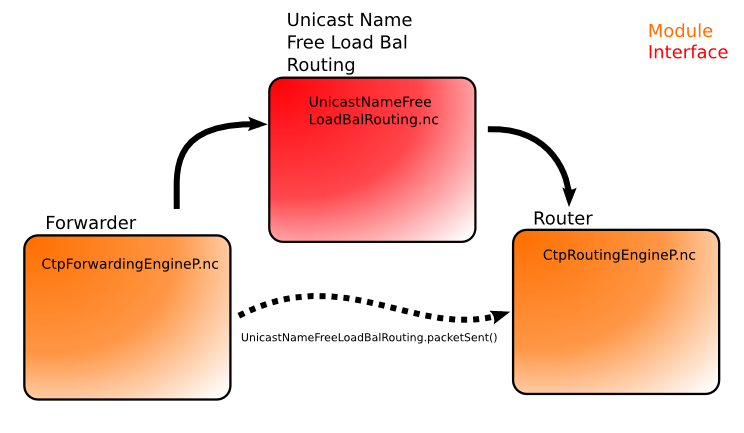
\includegraphics[width=0.75\textwidth]{Images/Components.png}
        }
    \end{block}
  }
\end{frame}





\section{Implementation}
\subsection{Code}

\begin{frame}[fragile]
  \frametitle{Our Design}
  \begin{itemize}
    \item $p^* = \text{arg min}  p \in \{\ \text{direct neighbours} \}\
                 [\alpha  \cdot (ETX_{s,p} + ETX_p) + \beta \cdot L_p^s]$

    \item Our design is to keep $L_p^s$ locally
  \end{itemize} 
   
  \footnotesize{
  \begin{block}{Code Implementation}
    \begin{verbatim}
// ETX for load balancing                                                                                                                                                              
uint16_t loadEtx;

//Complete Equation:
beaconMsg->etx = routeInfo.etx + 
call LinkEstimator.getLinkQuality(routeInfo.parent) 
+ (loadEtx/LOAD_EFFECT_THRESHOLD);
    \end{verbatim}
  \end{block}
}
\end{frame}

\begin{frame}[fragile]
  \frametitle{$t_p^s$}
  \footnotesize{
    \begin{block}{Code Implementation}
      \begin{verbatim}
/* 
 * Timer for the load balancing algorithm
 */
event void LoadTimer.fired() {
  //First decrement loadEtx to ensure decay
  if (loadEtx > 0) {
    loadEtx--;
  }
  //If there is a large change in loadEtx tell nabours
  if (radioOn && running) {
    if (loadEtx > oldLoadEtx + 10 || 
        (oldLoadEtx > 10 && loadEtx < oldLoadEtx - 10)) {
      post sendBeaconTask();
    }
  }
}
      \end{verbatim}
    \end{block}
  }
\end{frame}

\begin{frame}[fragile]
  \frametitle{$n_p^s$}
  \footnotesize{
    \begin{block}{Code Implementation}
      \begin{verbatim}
/*
 * This is to be called when ever a packet is sent via the radio.
 */
command void Routing.packetSent() {
  loadEtx++;
  printf("P\n");
  //printf("Load ETX Incremented. It is now: %d\n",loadEtx);
  //printfflush();
}
      \end{verbatim}
    \end{block}
  }
\end{frame}


\begin{frame}[fragile]
  \frametitle{Parameter Definitions}
  In TreeRouting.h:
  \footnotesize{
    \begin{block}{Code Implementation}
      \begin{verbatim}
enum {
    ...

    // Load balancing timer
    LOAD_INTERVAL = 100,        

    //Number of packets per rollover
    LOAD_EFFECT_THRESHOLD = 1, 

    ...
}; 
      \end{verbatim}
    \end{block}

    \begin{itemize}
      \item This allowed for easy access of values during the testing stage
    \end{itemize}
  }
\end{frame}


\section{Figures}
\subsection{CTP}

\begin{frame}[fragile]
  \frametitle{Initialisation}
  \footnotesize{
    \begin{block}{Data flow}
        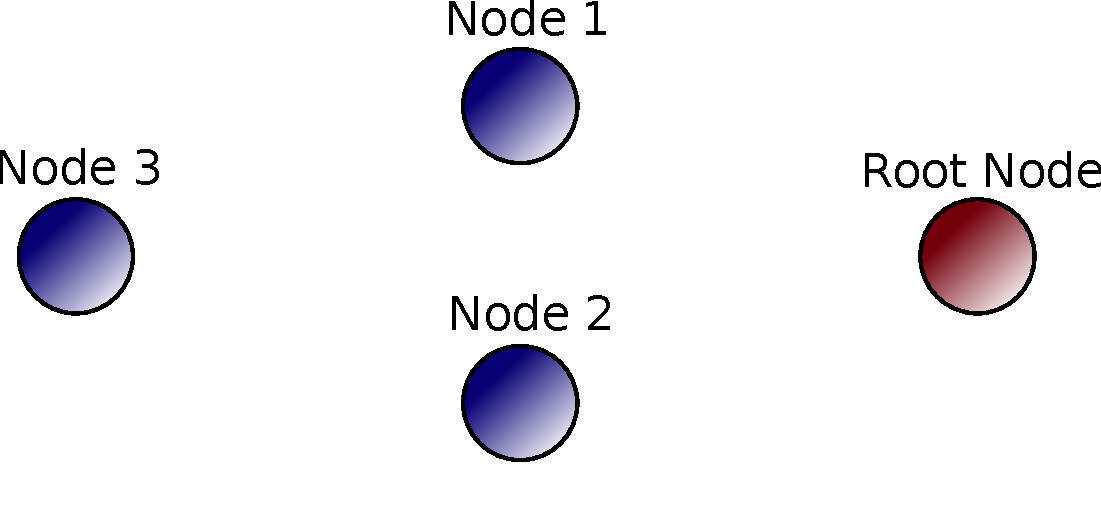
\includegraphics[width=\textwidth]{Images/Demo_plain}
    \end{block}
  }
\end{frame}


\begin{frame}[fragile]
  \frametitle{Initial route}
  \footnotesize{
    \begin{block}{Data flow}
        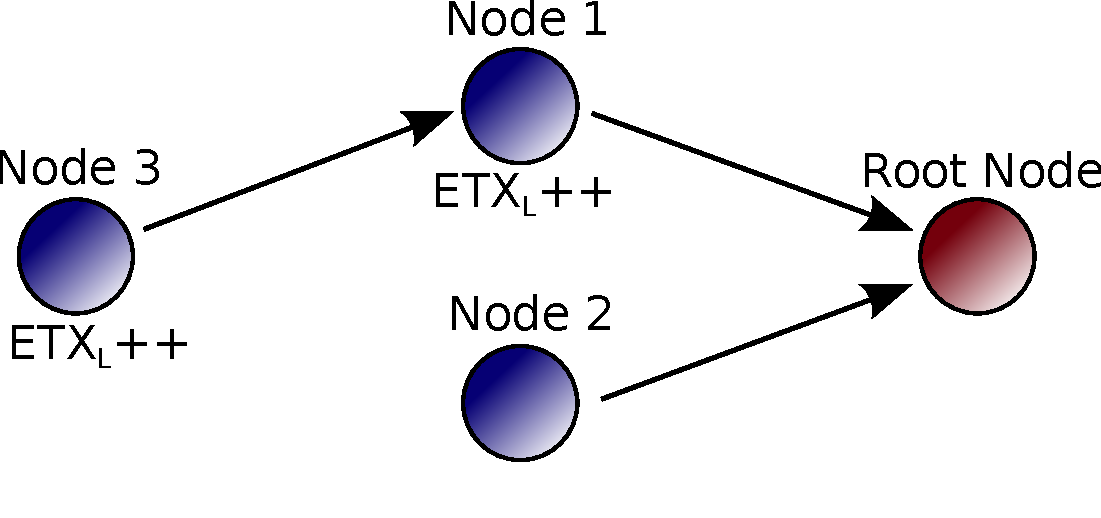
\includegraphics[width=\textwidth]{Images/Demo_s1}
    \end{block}
  }
\end{frame}

\begin{frame}[fragile]
  \frametitle{Load balanced}
  \footnotesize{
    \begin{block}{Data flow}
        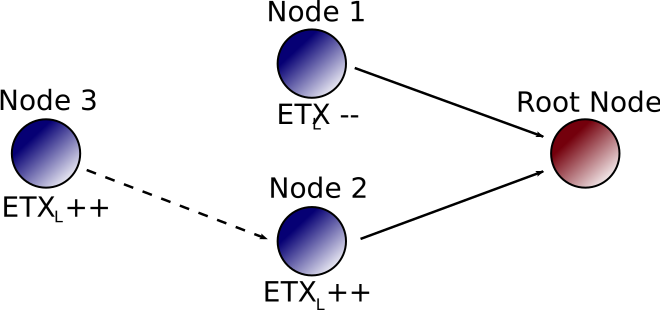
\includegraphics[width=\textwidth]{Images/Demo_s2}
    \end{block}
  }
\end{frame}


\begin{frame}[fragile]
  \frametitle{Load balanced (again)}
  \footnotesize{
    \begin{block}{Data flow}
        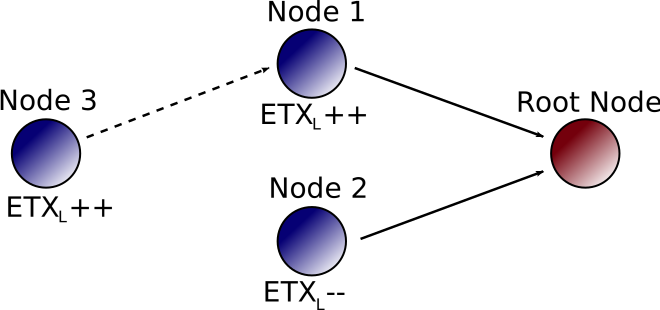
\includegraphics[width=\textwidth]{Images/Demo_s3}
    \end{block}
  }
\end{frame}

\section{Results \& Conclusions}
\subsection{Testing}

\begin{frame}
  \frametitle{Testing}
  \begin{itemize}
    \item Using lower transmit power
    \item \emph{printf} client to debug
    \item Listen client to view raw traffic
    \item Transmitting routing beacon every data packet
    \item Couldn't get Multihop oscilloscope working
    \item MViz showed our shifting ETX values
  \end{itemize}
\end{frame}  

\subsection{Conclusions}

\begin{frame}
  \frametitle{Conclusion}
  \begin{itemize}
    \item Still working on finding correct thresholds
    \item Currently implementing and testing code
    \item Can visualise operation using the MViz application
    \item We have implemented load balancing as a component to plug into
    standard CTP
    \item Simply include our CTP to use
  \end{itemize}
\end{frame}  


\end{document}
